\documentclass[aspectratio=169]{beamer}
\usepackage[UKenglish]{babel}
\usepackage[T1]{fontenc} % fontenc mit T1 sorgt für richtige Kodierung europäischer Zeichen
\usepackage[utf8]{inputenc} % Eingabezeichensatz: direkte Eingabe von Umlauten usw.
 % Anpassung des Dokumants deutsche Richtlinien

\usepackage{url} %Einbinden von Hyperlinks
\usepackage{mdwlist} % Für Listen ohne Abstand zwischen den Aufzählungspunkten.
\usepackage{paralist} % Ermöglicht Anpassung der Listen, z.B. Wahl des Autfählungszeichens

\usepackage{setspace} % Anpassung des Zeilenabstandes, Befehl muss vor der Berechnung des Satzspiegels gesetzt werden.

\usepackage{varioref} %Querverweise mit Seitenreferenz
\usepackage{fancyref} %Querverweise mit Angabe des Typs
\usepackage{xcolor}

%\usepackage[table,gray]{xcolor} %Zum Deaktivieren von Schattierung -- nur bei Verwendung des Packets "listings"
%\usepackage{listings} %Zur EInbindung von Quellcode verschiednester Art
\usepackage[locale=DE]{siunitx} % Korrekte Angabe von Einheiten
\usepackage[version=4]{mhchem}  % Für chemische Strukturformeln und Reaktionsgleichungen


\usepackage{booktabs} %Zur eleganten Formatierung von Tabellen
\usepackage{tabularx}
\usepackage{multirow} %Wenn man mehrere Zellen horizontal verbinden möchte

\beamertemplatenavigationsymbolsempty

%\setbeamertemplate{footline}[text line]{%
%\parbox{\linewidth}{\vspace*{-8pt}Laser cooling\hfill\insertshortauthor\hfill\insertpagenumber}}

\useoutertheme{infolines}
\usecolortheme{beaver}

\title{F61: Nuclear Magnetic Resonance}
\author{Alexander Impertro und Timo Gierlich}
\date{}

%*********************************************************************
% Document begins
%*********************************************************************

\begin{document}

\section{Chemical shift}

\subsection{Theory}

\begin{frame}
	\frametitle{Chemical shift -- theory}
	\begin{center}
		\textbf{Ziel:} structure determination of chemical substances
	\end{center}
	\pause
	\begin{columns}
		\column{.5\textwidth}
		\begin{itemize}
			\item electron orbitals contribute to $B_0$:
			\[\delta \vec{B} = \sigma \vec{B_0} \]
			\item modification of the Larmor frequency:
			\[ \omega_i = \omega_L \left(1-\sigma_i \right) \]
		\end{itemize}
      
		\column{.5\textwidth}
		\pause
		\begin{itemize}
			\item reference substance: TMS (Tetra-Methyl-Silan) 
			
			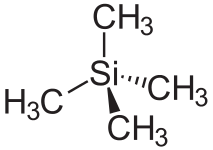
\includegraphics[width = 0.3\textwidth]{./Resources/Tetramethylsilan.png}
			\item relative chemical shift in ppm:
			\[ \delta_i = \sigma_i -\sigma_{TMS} = \frac{\omega_{TMS} - \omega_i}{\omega_L} \]
		\end{itemize}
	\end{columns}
\end{frame}

\begin{frame}
	\frametitle{Chemical shifts $\delta_i$ of compounds relative to TMS}

	\begin{center}
		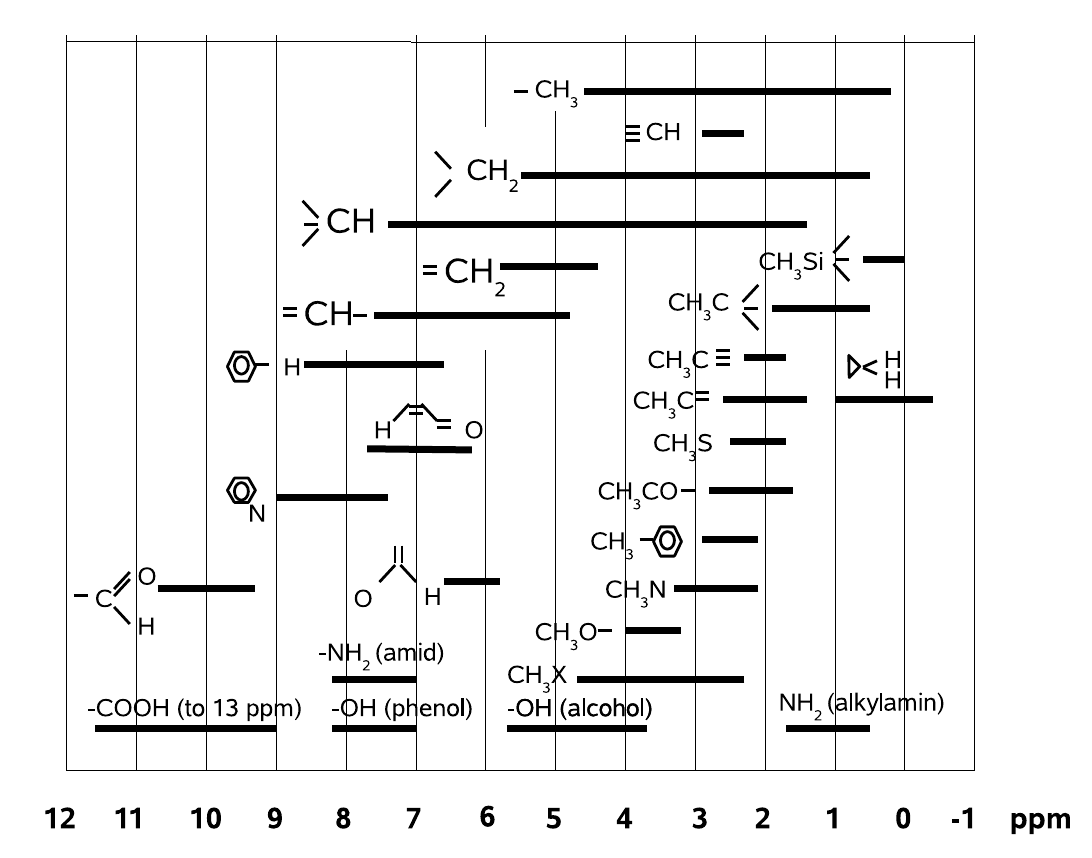
\includegraphics[width= 0.55\textwidth]{./Resources/chem_shifts.png}
	\end{center}
\end{frame}

\subsection{Measurements}

\begin{frame}
	\frametitle{Measurements}
		\begin{itemize}
			\item five chemical substances, with and without TMS
			\item inhomogeneities and diffusion processes reduce resolution
			
			$\Rightarrow$ thin glass tube, put into rotation with pressure air
			\item result:
			\begin{itemize}
				\item without rotation: 
				
				FWHM = \SI{200}{Hz}, I = 0,25
				\item with rotation: 
				
				FWHM = \SI{20}{Hz}, I = 1,9
			\end{itemize}
			\item energy resolution: 
			
			$\Delta E_{NMR} = h \cdot \Delta \nu = 8,28 \cdot 10^{-14} \, \mathrm{eV}$
		\end{itemize}
\end{frame}

\begin{frame}
	\frametitle{Idenfication of the Probes}
	\begin{center}
		\textbf{Probe C: acetic acid} 
\includegraphics[height = 0.6 cm]{./Resources/acetic_acid.png}	
	\end{center}
	
	\begin{table}[!htb]
		\centering
		%\caption{Messergebnisse für Probe C, Zuordnung: \emph{Essigsäure} }
		%\label{tab:Probe_C}
		\begin{tabular}{cccl}
			\toprule
			Peaks of C+ [ppm] & Peaks of C [ppm] & Chem. shift. &  \\
			\midrule
			$p_1 = 16,7$ & $p_1 = 17,0$ & $\delta_i = 11,6$ & \ce{COOH}-group \\

			$p_2 = 26,2$ & $p_2 = 26,6$ & $\delta_i = 2,1$ & Methyl group \ce{CH3} \\

			$p_3 = 28,3$ & -- & -- & TMS \\
			\bottomrule
		\end{tabular}
	\end{table}

\end{frame}

\begin{frame}
	\frametitle{Idenfication of the Probes}
	\begin{center}
		\textbf{Probe B: p-Xylol} 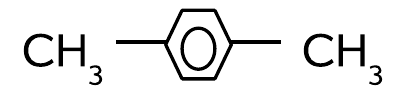
\includegraphics[height = 0.6 cm]{./Resources/p-xylol.png}
	\end{center}
	
	\begin{table}[!htb]
		\centering
	%\caption{Messergebnisse für Probe B, Zuordnung: \emph{p-Xylol} }
	%\label{tab:Probe_B}
		\begin{tabularx}{0.92\linewidth}{cccX}
			\toprule
			Peaks of B+ [ppm] & Peaks of B [ppm] & Chem. shift &  \\
			\midrule
			$p_1 = 22,7$ & $p_1 = 22,7$ & $\delta_i = 7,0$ & Benzene group \\

			$p_2 = 27,5$ & $p_2 = 27,5$ & $\delta_i = 2,2$ & Methyl group, Peak twice as high as $p_1$ \\

			$p_3 = 29,7$ & -- & --  & TMS \\

			\bottomrule
		\end{tabularx}
	\end{table}	

\end{frame}

\begin{frame}
	\frametitle{Idenfication of the Probes}
	\begin{center}
		\textbf{Probe E: toluol} 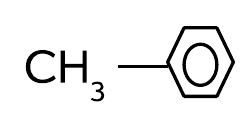
\includegraphics[height = 0.6 cm]{./Resources/toluol.png}
	\end{center}
	
	\begin{table}[!htb]
		\centering
%	\caption{Messergebnisse für Probe E, Zuordnung: \emph{Toluol} }
%	\label{tab:Probe_E}
		\begin{tabularx}{.92\linewidth}{cccX}
			\toprule
			Peaks of E+ [ppm] & Peaks of E [ppm] & Chem. shift &  \\
			\midrule
			$p_1 = 19,5$ & $p_1 = 23,1$ & $\delta_i = 7,3 $ & Benzene group \\

			$p_2 = 24,4$ & $p_2 = 23,1$ & $\delta_i = 2,4$ & Methyl group, peaks have same hight \\

			$p_3 = 26,8$ & -- & -- & TMS \\

			\bottomrule
		\end{tabularx}
	\end{table}
	
\end{frame}



\begin{frame}
	\frametitle{Idenfication of the Probes}
	\begin{center}
		\textbf{Probe A: fluoroaceton} 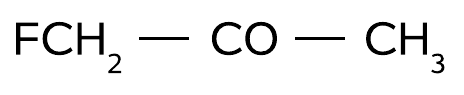
\includegraphics[height = 0.6 cm]{./Resources/fluoroacetone.png}
	\end{center}
	
	\begin{table}[!htb]
		\centering
		%\caption{Messergebnisse für Probe A, Zuordnung: \emph{Flouraceton} }
		%\label{tab:Probe_A}
		\begin{tabularx}{.90\linewidth}{cccX}
			\toprule
			Peaks of A+ [ppm] & Peaks of A [ppm] & Chem. shift &  \\
			\midrule
			$p_1 = 22,2$ & $p_1 = 23,8$ & $\delta_i = 6,3$ & \multirow{2}{*}{\ce{FCH2}-group} \\

			$p_2 = 24,6$ & $p_2 = 21,4$ & $\delta_i= 3,9$ &  \\

			$p_3 = 26,4$ & $p_3 = 19,6$ & $\delta_i = 2,1 $ & Methyl group \ce{CH3} \\

			$p_4 = 28,5$ & -- & -- & TMS \\
			\bottomrule
		\end{tabularx}
	\end{table}
	
\end{frame}

\begin{frame}
	\frametitle{Idenfication of the Probes}
	\begin{center}
		\textbf{Probe D: fluoroacetonitril} 
\includegraphics[height = 0.6 cm]{./Resources/fluoroacetonitril.png}
	\end{center}
	
	\begin{table}[!htb]
		\centering
%	\caption{Messergebnisse für Probe D, Zuordnung: \emph{Fluoroacetonitril} }
%	\label{tab:Probe_D}
		\begin{tabularx}{.9\linewidth}{cccX}
			\toprule
			Peaks of D+ [ppm] & Peaks of D [ppm] & Chem. shift &  \\
			\midrule
			$p_1 = 30,8$ & -- & -- & TMS \\

			$p_2 = 34,8$ & $p_2 = 26,6$ & $\delta_i = 6,4$ & \multirow{2}{*}{\ce{FCH2} group} \\

			$p_3 = 37,2$ & $p_3 = 24,2$ & $delta_i = 4,0$ &  \\

			\bottomrule
		\end{tabularx}
	\end{table}
\end{frame}

\section{Imaging with NMR}

\subsection{Theory}

\subsubsection{one dimensional imaging}

\begin{frame}
	\frametitle{one dimensional imaging -- theory}
	\begin{itemize}
		\item \textbf{position dependent magnet fields}
		\item Superposition of the static field $\vec{B_0}$ with gradient fields $\vec{B^x}$, $\vec{B^y}$, $\vec{B^z}$
		\item two techniques:
	\end{itemize}
	\begin{columns}
		\column{.5\textwidth}
			\begin{description}
				\item[frequency coding]
			\end{description}
			\begin{itemize}
				\item Larmor frequency $\omega_L = \gamma (B_0 + G^z \cdot z) = \omega_L^0 + \omega_z$
				\item measured NMR signal $S(t)$ is Fourier transform of $M_{\perp}^{rot}(z)$
			\end{itemize}
		\column{.5\textwidth}
			\begin{description}
				\item[phase coding]
			\end{description}
			\begin{itemize}
				\item apply gradient field, increase strength
				\item phase rotates: $\phi (z) = (\gamma G^z T_{Ph})z = k_z z$
			\end{itemize}
			
	\end{columns}	
\end{frame}

\begin{frame}
	\frametitle{two dimensional imaging -- theory}
	\begin{center}
		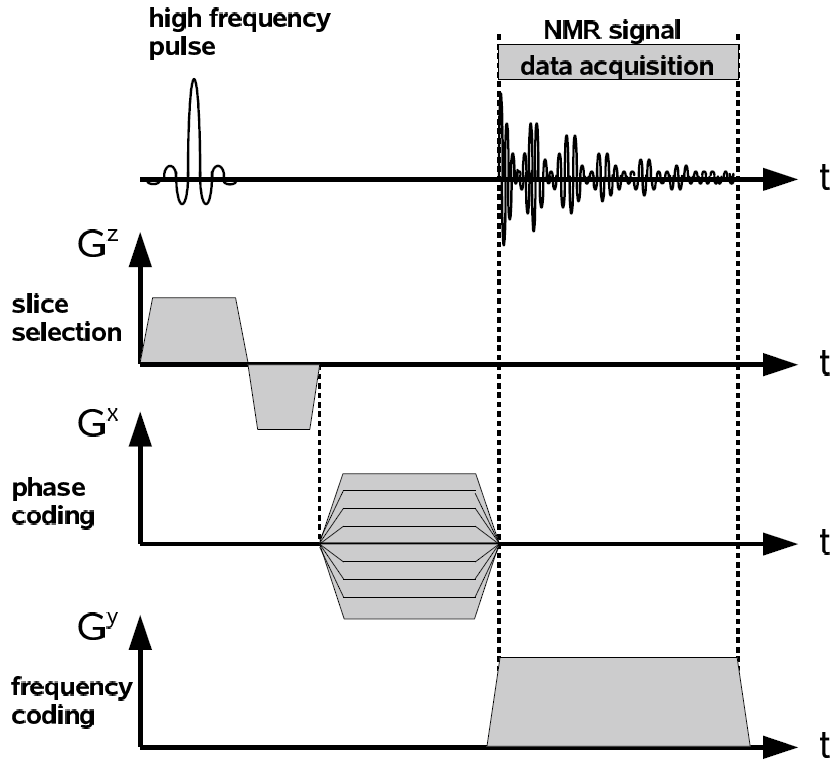
\includegraphics[width=0.4\linewidth]{./Resources/2d_imaging.png}
	\end{center}

\end{frame}

\subsection{Experiments}

\subsubsection{one dimensional imaging}

\begin{frame}
	\frametitle{One dimensional imaging measurements}
	\begin{columns}
		\column{.5\textwidth}
		\begin{itemize}
			\item Bruker$^{\textregistered}$ NMR analyzer mq7.5
			\item Glass tube filled with \SI{15}{mm} of oil
			\item Glass tube filled with \SI{50}{mm} of water
			\item glass tube with teflon structure
			\item examination of an inflitration process: 
			
			Fick's second law: $\frac{\partial c}{\partial t} = D \frac{\partial^2 c}{\partial x^2}$
		\end{itemize}
		
		\column{.5\textwidth}
		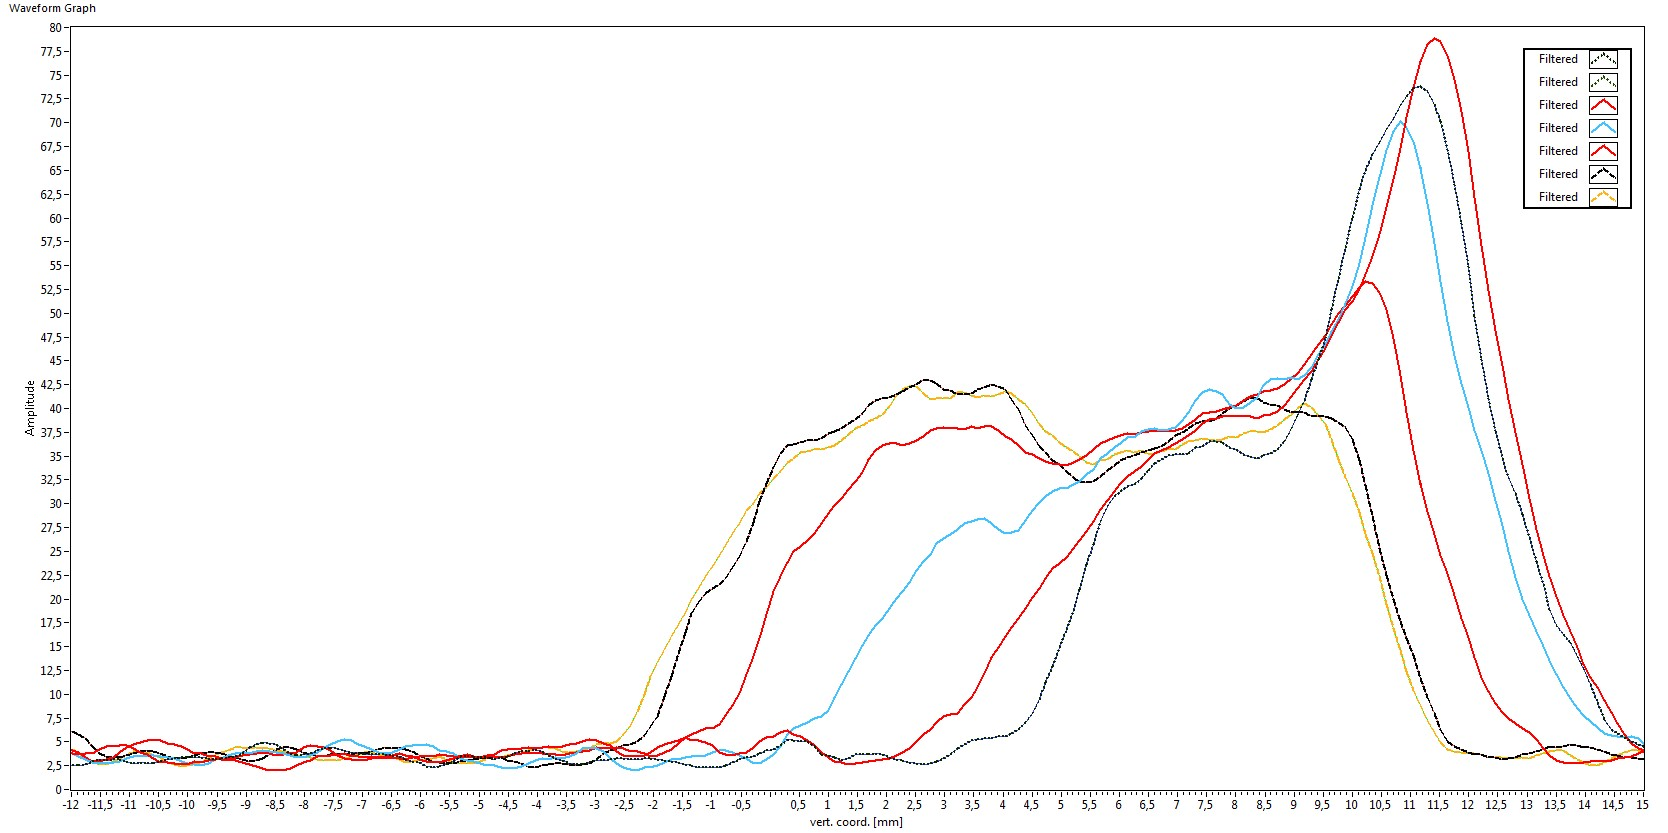
\includegraphics[width=1.0 \linewidth]{./Resources/Teil_3/oeldiff_chinchilla.jpg}
	\end{columns}	
\end{frame}

\subsubsection{two dimensional imaging}

\begin{frame}
	\frametitle{two dimensional imaging measurements}
	\begin{columns}
		\column{.5\textwidth}
		\begin{figure}
			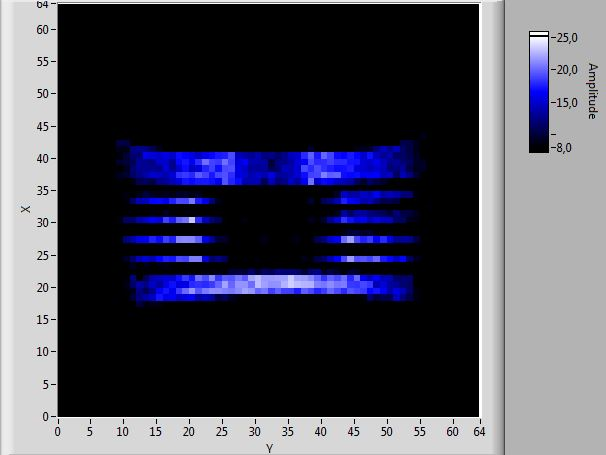
\includegraphics[width=.80 \linewidth]{./Resources/Teil_3/ptfe_vert.JPG}
			\caption{teflon structure}
		\end{figure}

		\column{.5\textwidth}
		\begin{figure}
			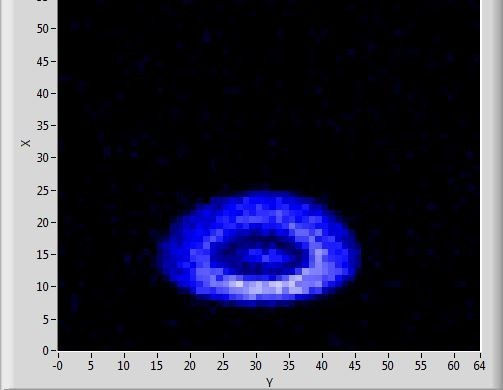
\includegraphics[width=0.8 \linewidth]{./Resources/Teil_3/olive_2d.JPG}
			\caption{olive}
		\end{figure}
		
	\end{columns}
\end{frame}

\begin{frame}
	\frametitle{two dimensional imaging measurements}
	\begin{columns}
		\column{.5\textwidth}
		\begin{figure}
			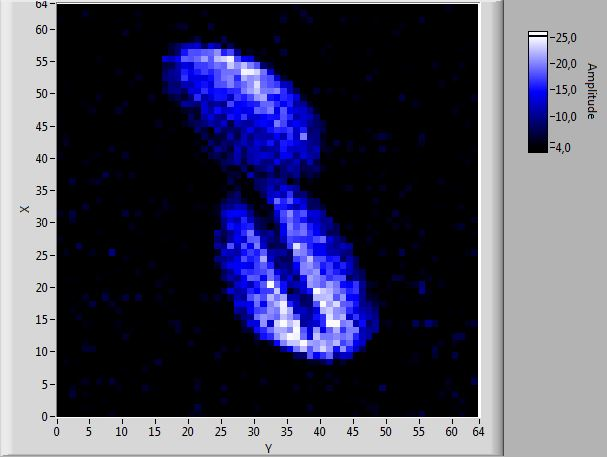
\includegraphics[width=.80 \linewidth]{./Resources/Teil_3/peanut_shell.JPG}
			\caption{peanut shell}
		\end{figure}

		\column{.5\textwidth}
		\begin{figure}
			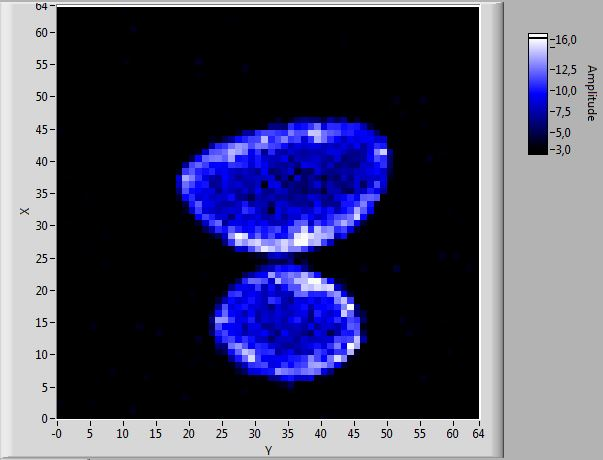
\includegraphics[width=0.8 \linewidth]{./Resources/Teil_3/aloevera_2d.JPG}
			\caption{aloe vera}
		\end{figure}
		
	\end{columns}
\end{frame}

\end{document}

